\section{Classifying Users of High Target Specificity}
\label{sec:ClassificationMethod2}

In this chapter, in regard to target users classified by the method
mentioned in the above chapter, we explain the method of determining why
their target specificity is high based on the result of our analysis
mentioned in \ref{subsec:The Causes}.

\subsection{Architecture of the Classifiers}
\label{subsec:Architecture}

Here, we focus on the two causes of high target specificity
mentioned in \ref{subsec:The Causes} as follows:
\begin{description}
 \item[(1)] because they publish information on some specific topics, and
 \item[(2)] because they publish information to a specific gropu of users,
\end{description}

\noindent{and we determine whether a user we intend to classify
correlates with each cause mentioned above.}

We first determine various features of the user which potentially
correlate with each cause.  Then, based on these features, we construct
the classification method which classifies users into three categories:
(1) their target specificity is high because they publish information
on some specific topics, (2) because they publish information to
a specific group of users, and (3) in the cause of both (1) and
(2).  By classifying users with the above method, we determine why
their target specificity is high.

We adopted SVM and the decision tree as a classifier.  Next, we propose a
couple of approaches to classify users into three categories.

\subsubsection{3-class Classifier}
\label{subsubsec:3-class}

In the first approach, we construct a single 3-class classifier using
one-against-one method.  Each result class corresponds to each category:
(1), (2), and (3).  Figure~\ref{fig:classifier} (a) shows the architecture
of a 3-class classifier.

\subsubsection{2 Binary Classifiers}
\label{subsubsec:2-binary}

In the second approach, we construct 2 binary classifiers, each of
which determines (i) whether users publish information on some specific
topics, and (ii) whether users publish information to a specific group
of users, respectively.  When the results of two
classifiers are \emph{yes} and \emph{no} respectively, we classify them
into the category (1): their target specificity is high because they
publish information on some specific topics.  When the results are
\emph{no} and
\emph{yes}, we classify them into the category (2): because they publish
information to a specific group of users, and when the results
are \emph{yes}
and \emph{yes}, we classify them into the category (3): in the cause of
both (1) and (2).  Figure~\ref{fig:classifier} (b) shows the architecture of
2 binary classifiers.

{\footnotesize
\begin{figure}[t]
\begin{center}
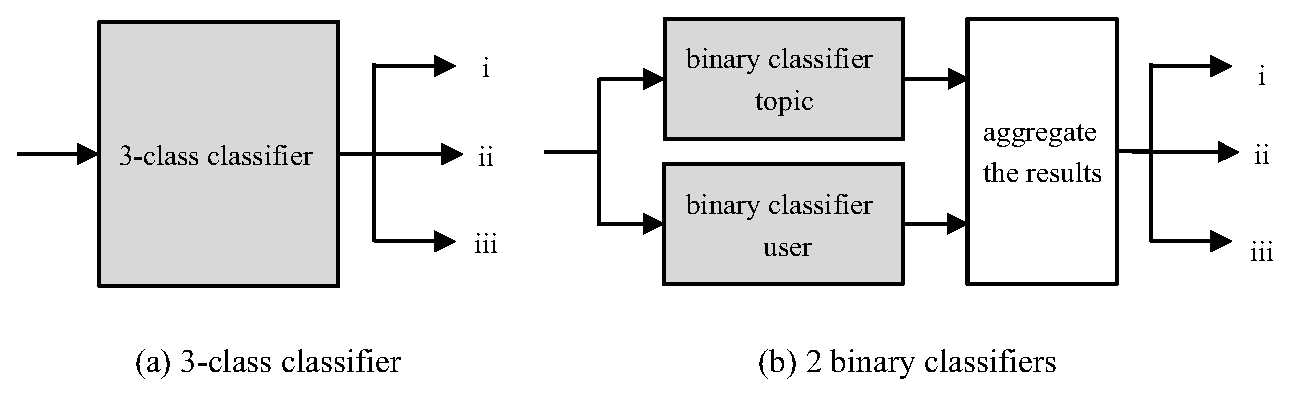
\includegraphics[width=14cm]{images/classifier.eps}
 \caption{Architecture of a couple of classifiers: (a) 3-class
 classifier and (b) 2 binary classifiers}
\label{fig:classifier}
\end{center}
\end{figure}
}

\subsection{Features Used for the Classification}
\label{subsec:Features}

In this subchapter, we explain what features of users we used for the
classification.  All the feature values shown below are normalized to
values between $0$ and $1$.

\begin{description}
\bf {\item[(i)] numbers of followees and followers, and their ratio}
\end{description}

If the user publishes information to unspecific users, there is a high
possibility that a number of his followers is quite large or a
number of his followees is quite small.  So in such a case, a ratio
of a number of his followees to a number of his followers is
supposed to be very small.  Furthermore, if the user publishes
information to the closed users, i.e., his friends, his club
members, and so on, there is a high possibility that numbers of his
followers and followees are very close because the user is supposed to
have a reciprocal connection with them.  Thus, numbers of followees and
followers, and their ratio are expected to be useful for determining why
their target specificity is high.

We take a logarithm of numbers of followers and followees because the
difference of large numbers of followers and followees are not as
important as the difference of small numbers of followers and followees.

\begin{description}
\bf {\item[(ii)] mutual follow ratio}
\end{description}

There is a high possibility that the user publishing information to the
closed users has a large mutual follow ratio, i.e., a number of users
with whom one follows one another is large, because the user is supposed
to have a reciprocal connection with them.  Therefore, a mutual follow
ratio is expected to be useful for determining why their target
specificity is high.

\begin{description}
\bf {\item[(iii)] frequency of replies by ``@''}
\end{description}

There is a high possibility that the user publishing information to the
closed users has a high frequency of replies by ``@'', i.e., the user
replies to his followers frequently. In regard to a mutual follow
ratio mentioned in the feature (ii), there are some users publishing information to
unspecified users in spite of a large mutual follow ratio, who are
called socializers.  But in regard to a frequency of replies by ``@'',
there is a high possibility that the
user publishes information to the closed users.  This is because a high
frequency of replies by ``@'' demonstrates that the user is supposed to
have a reciprocal connection with them.  Therefore, a frequency of
replies by ``@'' is expected to be useful for determining why their
target specificity is high.

\begin{description}
\bf {\item[(iv)] partialness of topics in messages}
\end{description}

In regard to a user publishing information on some specific topics,
topics in his messages are often partial.  Thus, we use the
partialness of topics in his messages as a feature for the
classification.

Then, we explain how to compute a partialness of topics in messages of
$u$.  We first collect up to the latest 200 messages from each user we
intend to classify.  Second,
we extract noun phrases from them and we use their phrases as a corpus.
We extract only noun phrases because they characterize contents of the
messages more strongly than other phrases.  Then, in regard to each user
$u$, we determine the topic of each message by
using Latent Dirichlet Allocation (LDA), which is a generative
probabilistic model for collections of discrete data such as text
corpora, by using the above corpus.  Finally, we compute the partialness of
topics in messages $\mathit{partialness}(u)$ as follows:

\vspace{-3ex}
\[
 \mathit{partialness}(u) = - \sum_{t \in T_u} p_t \log p_t,\;\;\;\;\;
 p_t = \frac{|\{m|\;m \in M_u,\;\mathit{topic}(m) = t\}|}{|M_u|}
\]
\vspace{-3ex}

\noindent{where $M_u$ is a message set of $u$, $T_u$ is the topic set we
use for computing this feature, and $\mathit{topic}(m)$ is the topic of
a message $m$.  The partialness of topics $partialness(u)$ is the
entropy of $M_u$ on the topic.  This is how we compute a partialness of
topics in messages.}